\documentclass[12pt,a4paper,oneside]{article}
\usepackage[colorlinks=true]{hyperref}
\usepackage[utf8]{inputenc}
\usepackage[english]{babel}
\usepackage{graphicx}
\usepackage{pdfpages}
\textwidth 16cm \textheight 25cm
\topmargin -1.3cm 
\oddsidemargin 0cm
\pagestyle{empty}
\begin{document}
\title{SDR meteor detector}
\author{Jakub Kákona, kaklik@mlab.cz }
\maketitle

\begin{abstract}
Construction of software defined radio meteor detector with possibility of advanced signal processing.
\end{abstract}

\begin{figure} [htbp]
\begin{center}
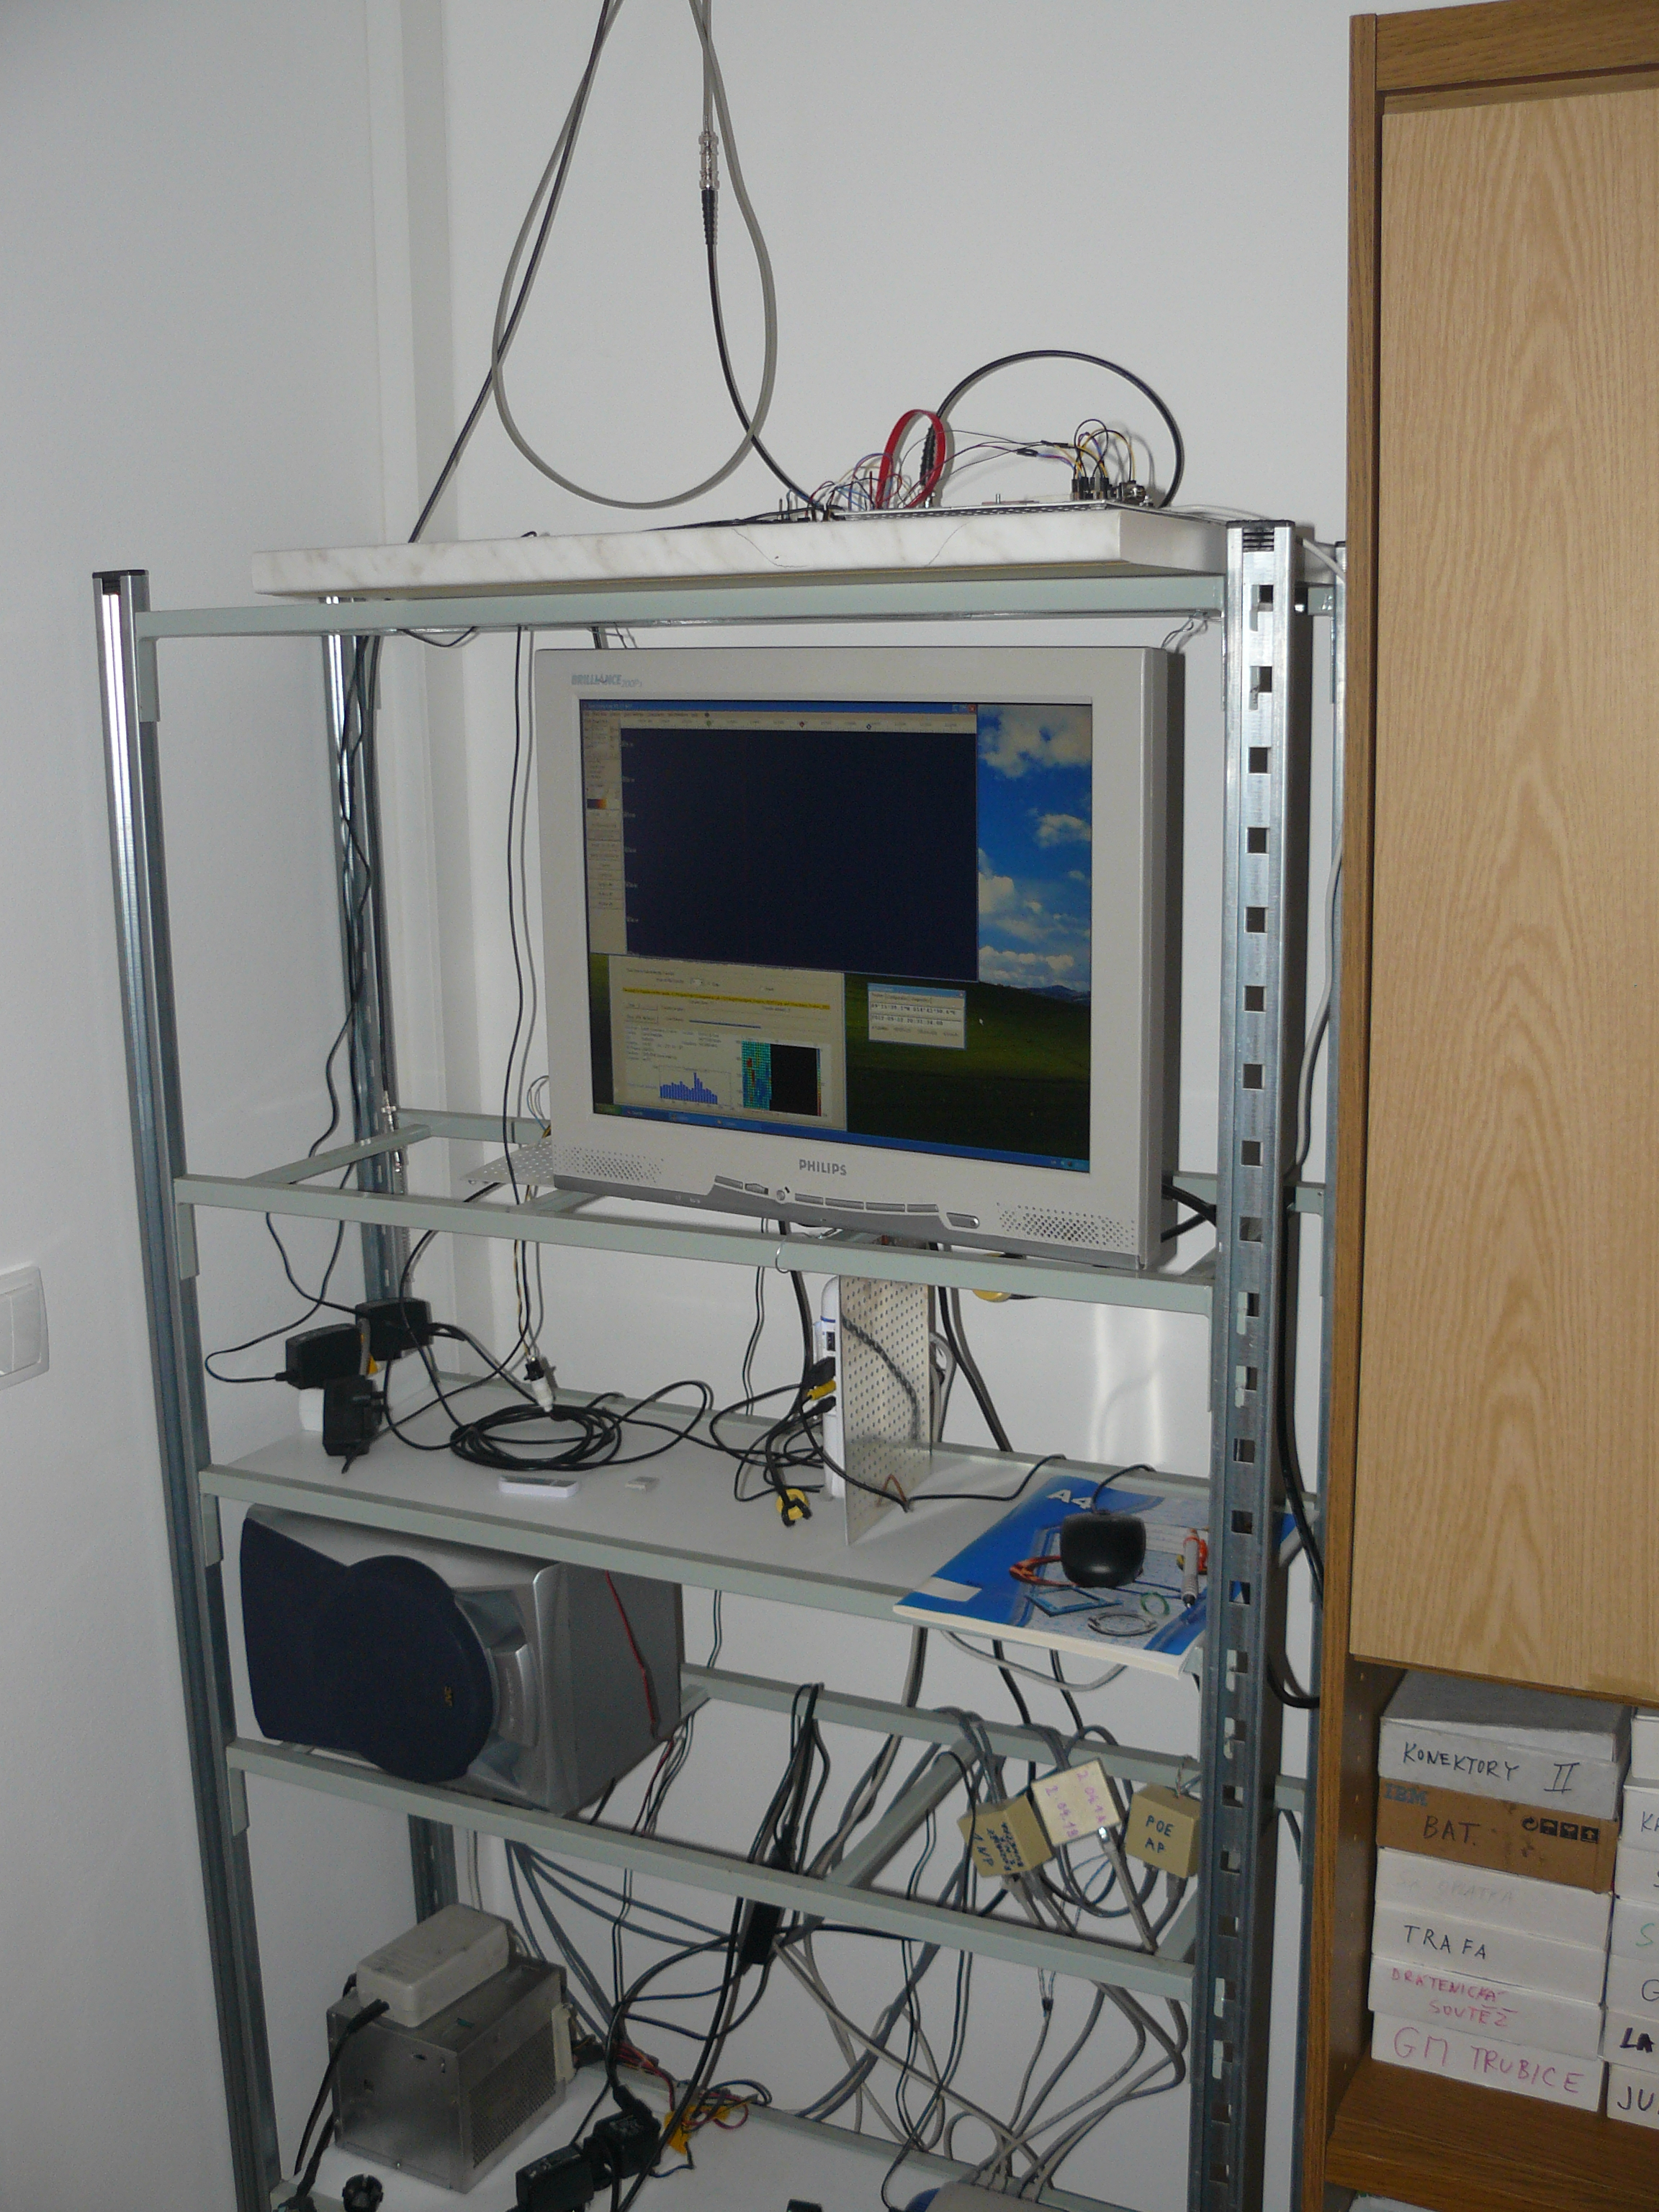
\includegraphics [width=80mm] {./img/meteor_detector_station.JPG} 
\end{center}
\end{figure}

\begin{figure} [b]

\includegraphics [width=25mm] {./img/SDRX01B_QRcode.png} 
\end{figure}

\newpage
\tableofcontents

\section{Technical parameters}
\begin{table}[htbp]
\begin{center}
\begin{tabular}{|c|c|p{5cm}|}
\hline
\multicolumn{1}{|c|}{Parameter} & \multicolumn{1}{|c|}{Value} & \multicolumn{1}{|c|}{Note} \\ \hline
Powering voltage for analogue part & $\pm$12V &  50mA \\ \hline
Powering voltage for digital part & +5V &  300mA \\ \hline
Bias of optional LNA & 9V &  500 mA maximum \footnote{Fused by 750mA on the reciver board} \\ \hline
Frequency range  & 0,5 - 200 MHz & Usually working at 143.05 MHz \\ \hline
Gain & 90dB & Selectable by jumper and LNA configuration \\ \hline
Self noise number & $<$ 30dB & \\ \hline
\end{tabular}
\end{center}
\end{table}

\newpage
\section{Introduction}

The detection of meteors by radio is most readily accomplished by a method known as "forward scatter".  This technique usually exploits the existence of a VHF radio transmitter intended for some other purpose (such as historically analogue radio or TV broadcasting) and which is preferably situated some way beyond the optical horizon so that the direct signal does not desensitise the receiving equipment.  The radio signal reflects mainly from the ionised meteor trail as it forms and dissipates, causing a brief signal to be heard on or close to the transmitter frequency.  The trails form in the ionosphere (i.e., the upper atmosphere) at a height of about 100 $\pm$ 20 km.

Direct reflection from the meteoroid itself  is not so readily detected.  Meteoroids are not necessarily reflective at radio frequencies, they are usually small (0.05 - 200mm) and they generally enter the ionosphere at supersonic velocities.  Thus the direct signal is usually weak; and the initial Doppler shift is  large, making it difficult to associate the signal with the transmitter.  Sometimes however, a Doppler shifted signal is observed to slew onto or across the transmitter frequency at the beginning of the detection event.  This is the reflection from the ball of plasma surrounding the meteoroid (as opposed to the trail left behind), and is known as the "head echo". 

     The term "radar" is sometimes used to describe the forward scatter detection method.  Note however, that 'radar' is an acronym for 'radio direction and ranging' and so, although distance and direction information can be extracted from data aggregated from an array of receivers, a single receiver installation does not constitute a radar system.  A single receiver can only strictly report an estimate of the number of meteoroids which enter the ionosphere in the region illuminated by the chosen radio transmitter.  Other interesting aspects of the meteor strike can be inferred from the recorded signals, but apparently obvious information, such as the relationship between signal strength and meteoroid mass is complicated by issues such as signal polarisation, trajectory and transmitter coverage. 
     
     One advantage of radio detection is that it works when the sky is light or when the sky is dark but overcast.  By choosing a sufficiently powerful host transmitter, it also possible to record meteors which are too faint for the human eye even in the darkest and clearest conditions.  A figure of between 2 and 10 times as many meteors as can be seen by visual observation under ideal conditions is sometimes quoted; but this must depend on the transmitter power and radiation pattern.

\section{Description of construction}

This construction of radio meteor detector uses France GRAVES space-surveillance radar. The radar has transmitting power of several megawatts at frequency 143.05 MHz.   

\subsection{Antenna}
The detector station usually uses  modified ground plane antenna. Adjusted in angle of 30$^\circ$ to East this configuration seems to be optimal to detecting stations in the Czech Republic. 

\begin{figure} [htbp]
\begin{center}
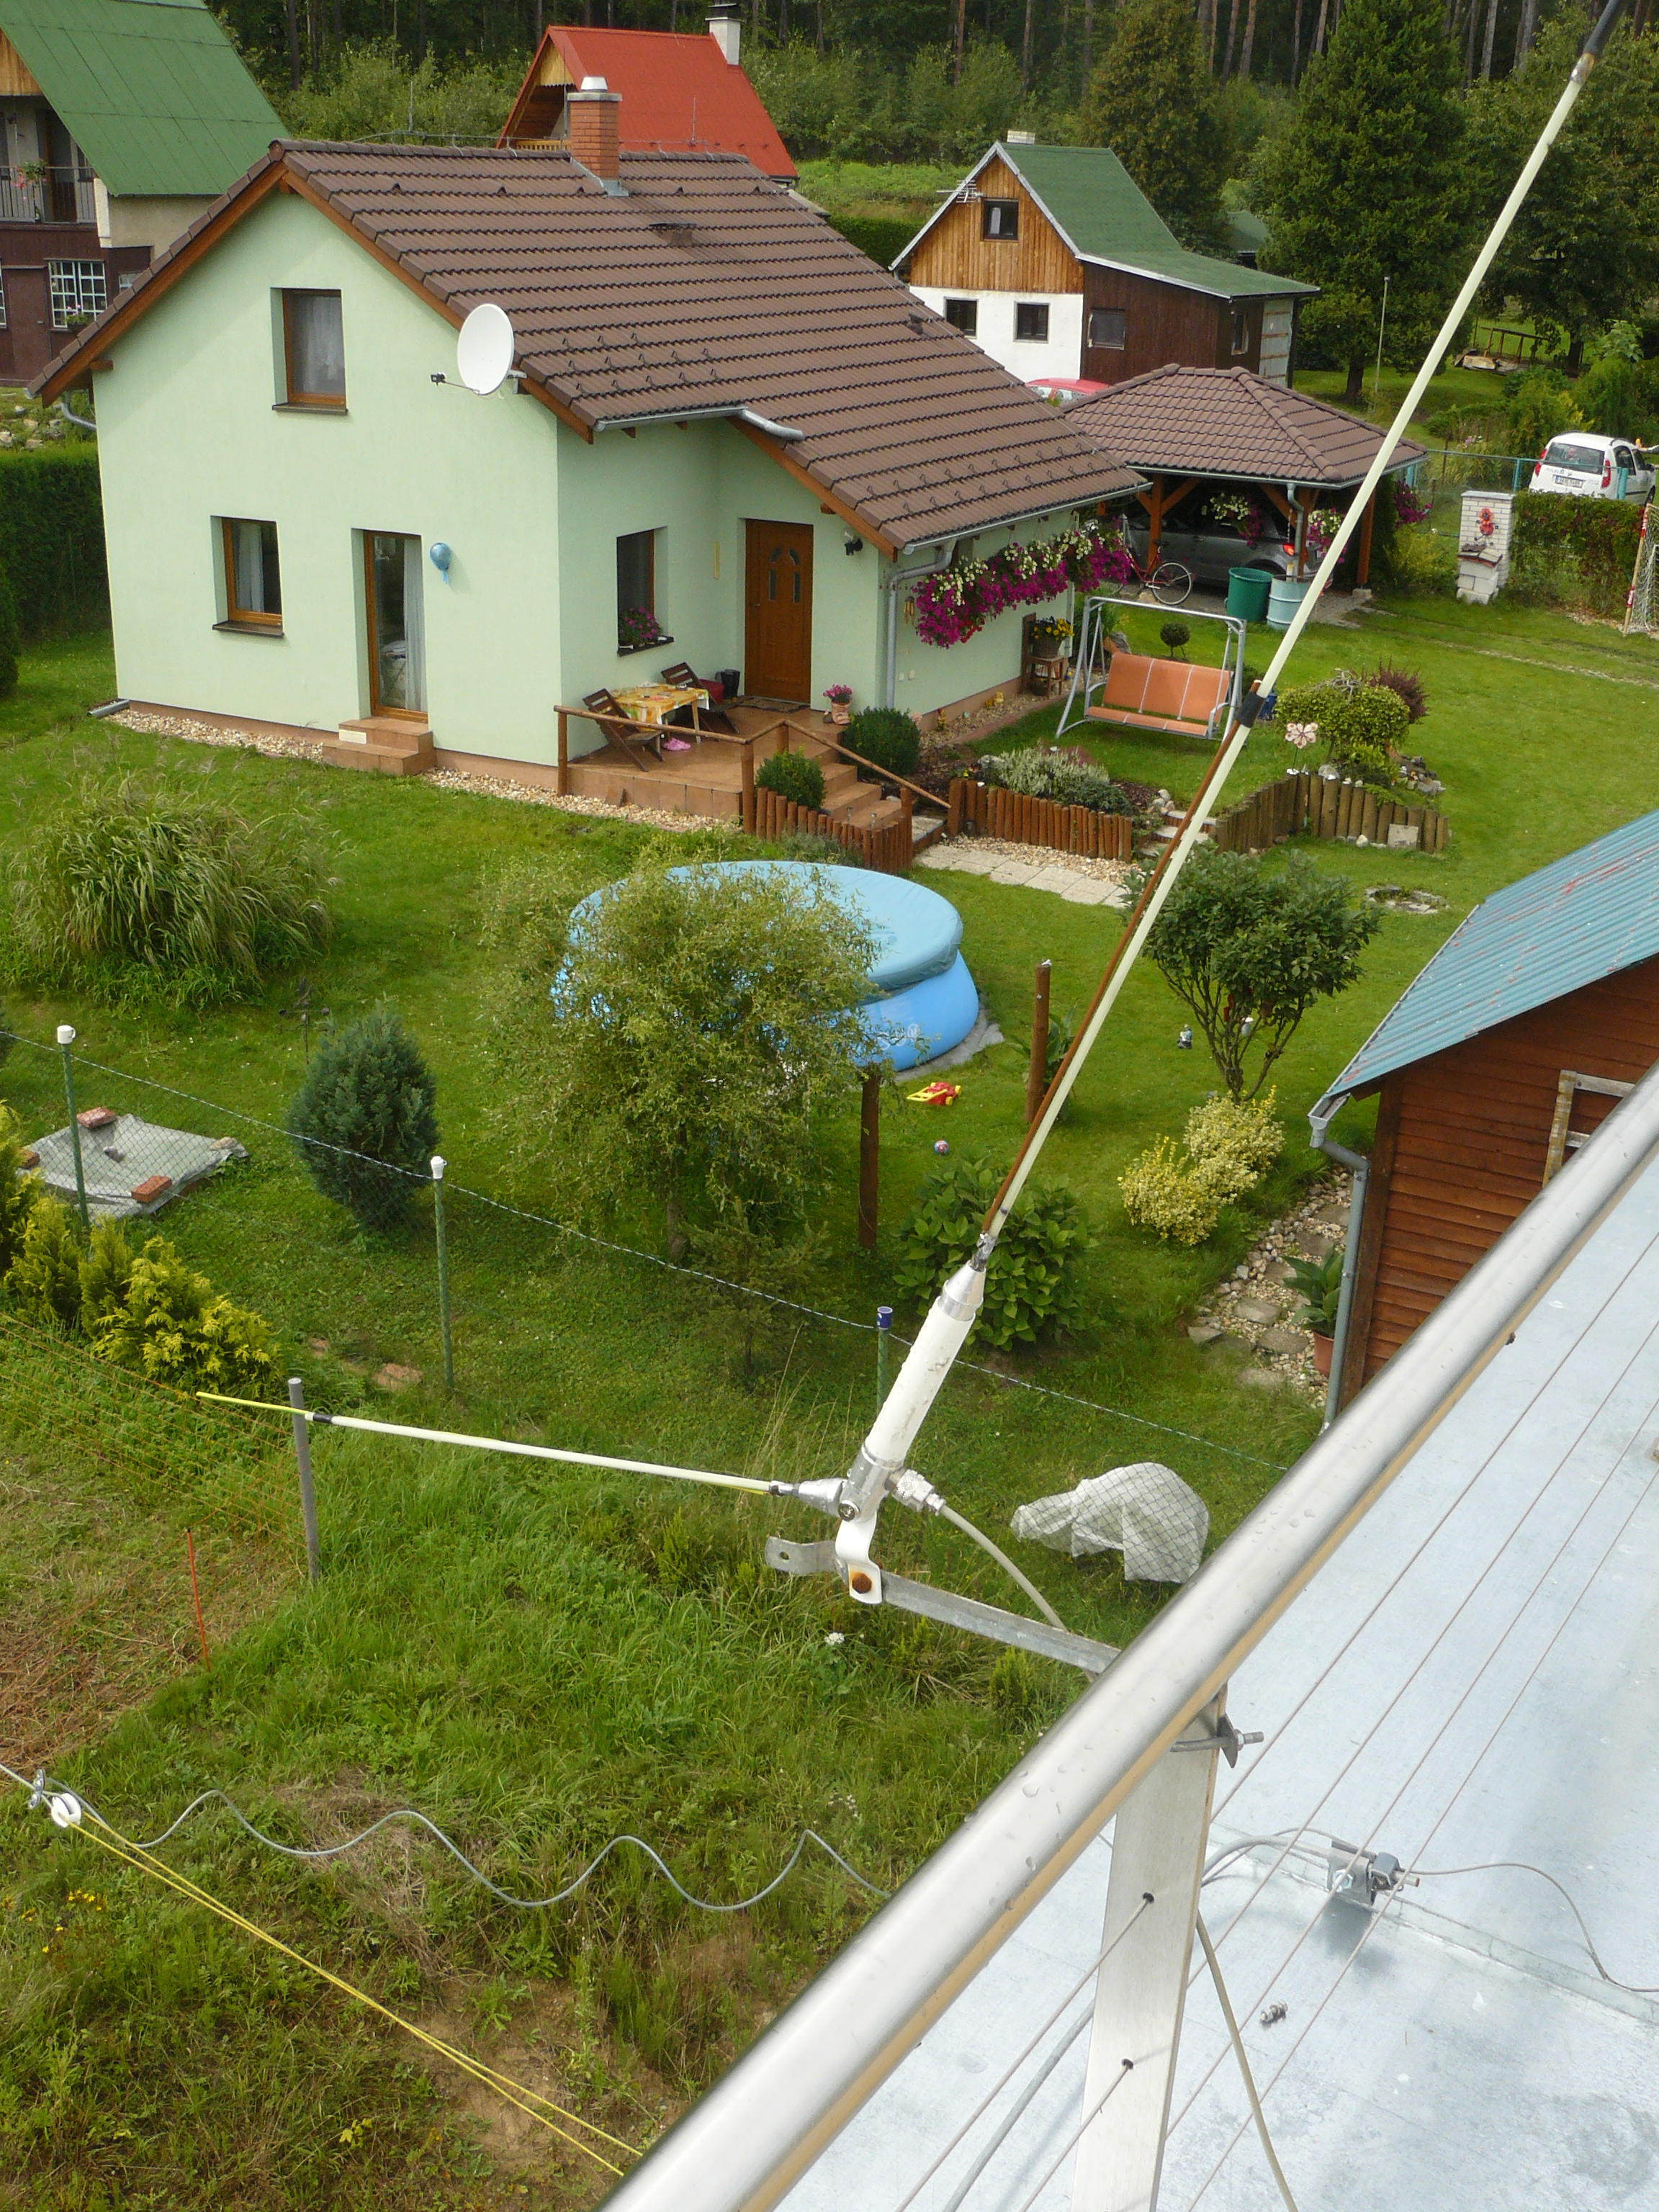
\includegraphics [width=80mm] {./img/GP143MHz.JPG} 
\end{center}
\caption{Antenna used at detection station}
\end{figure}

The received signal from antenna is amplified by specially constructed LNA. This step is needed for feeding the signal trough relative long (several metres) coax RG58. Construction of LNA01A is described on MLAB project site. 

\subsection{SDR receiver}

The SDR receiver used is MLAB system SDRX01B direct sampling receiver. This receiver has ideal performance for UHF and lower band radioastronomy.    So this receiver can be used even for radio meteor detection. 

\begin{figure} [htbp]
\begin{center}
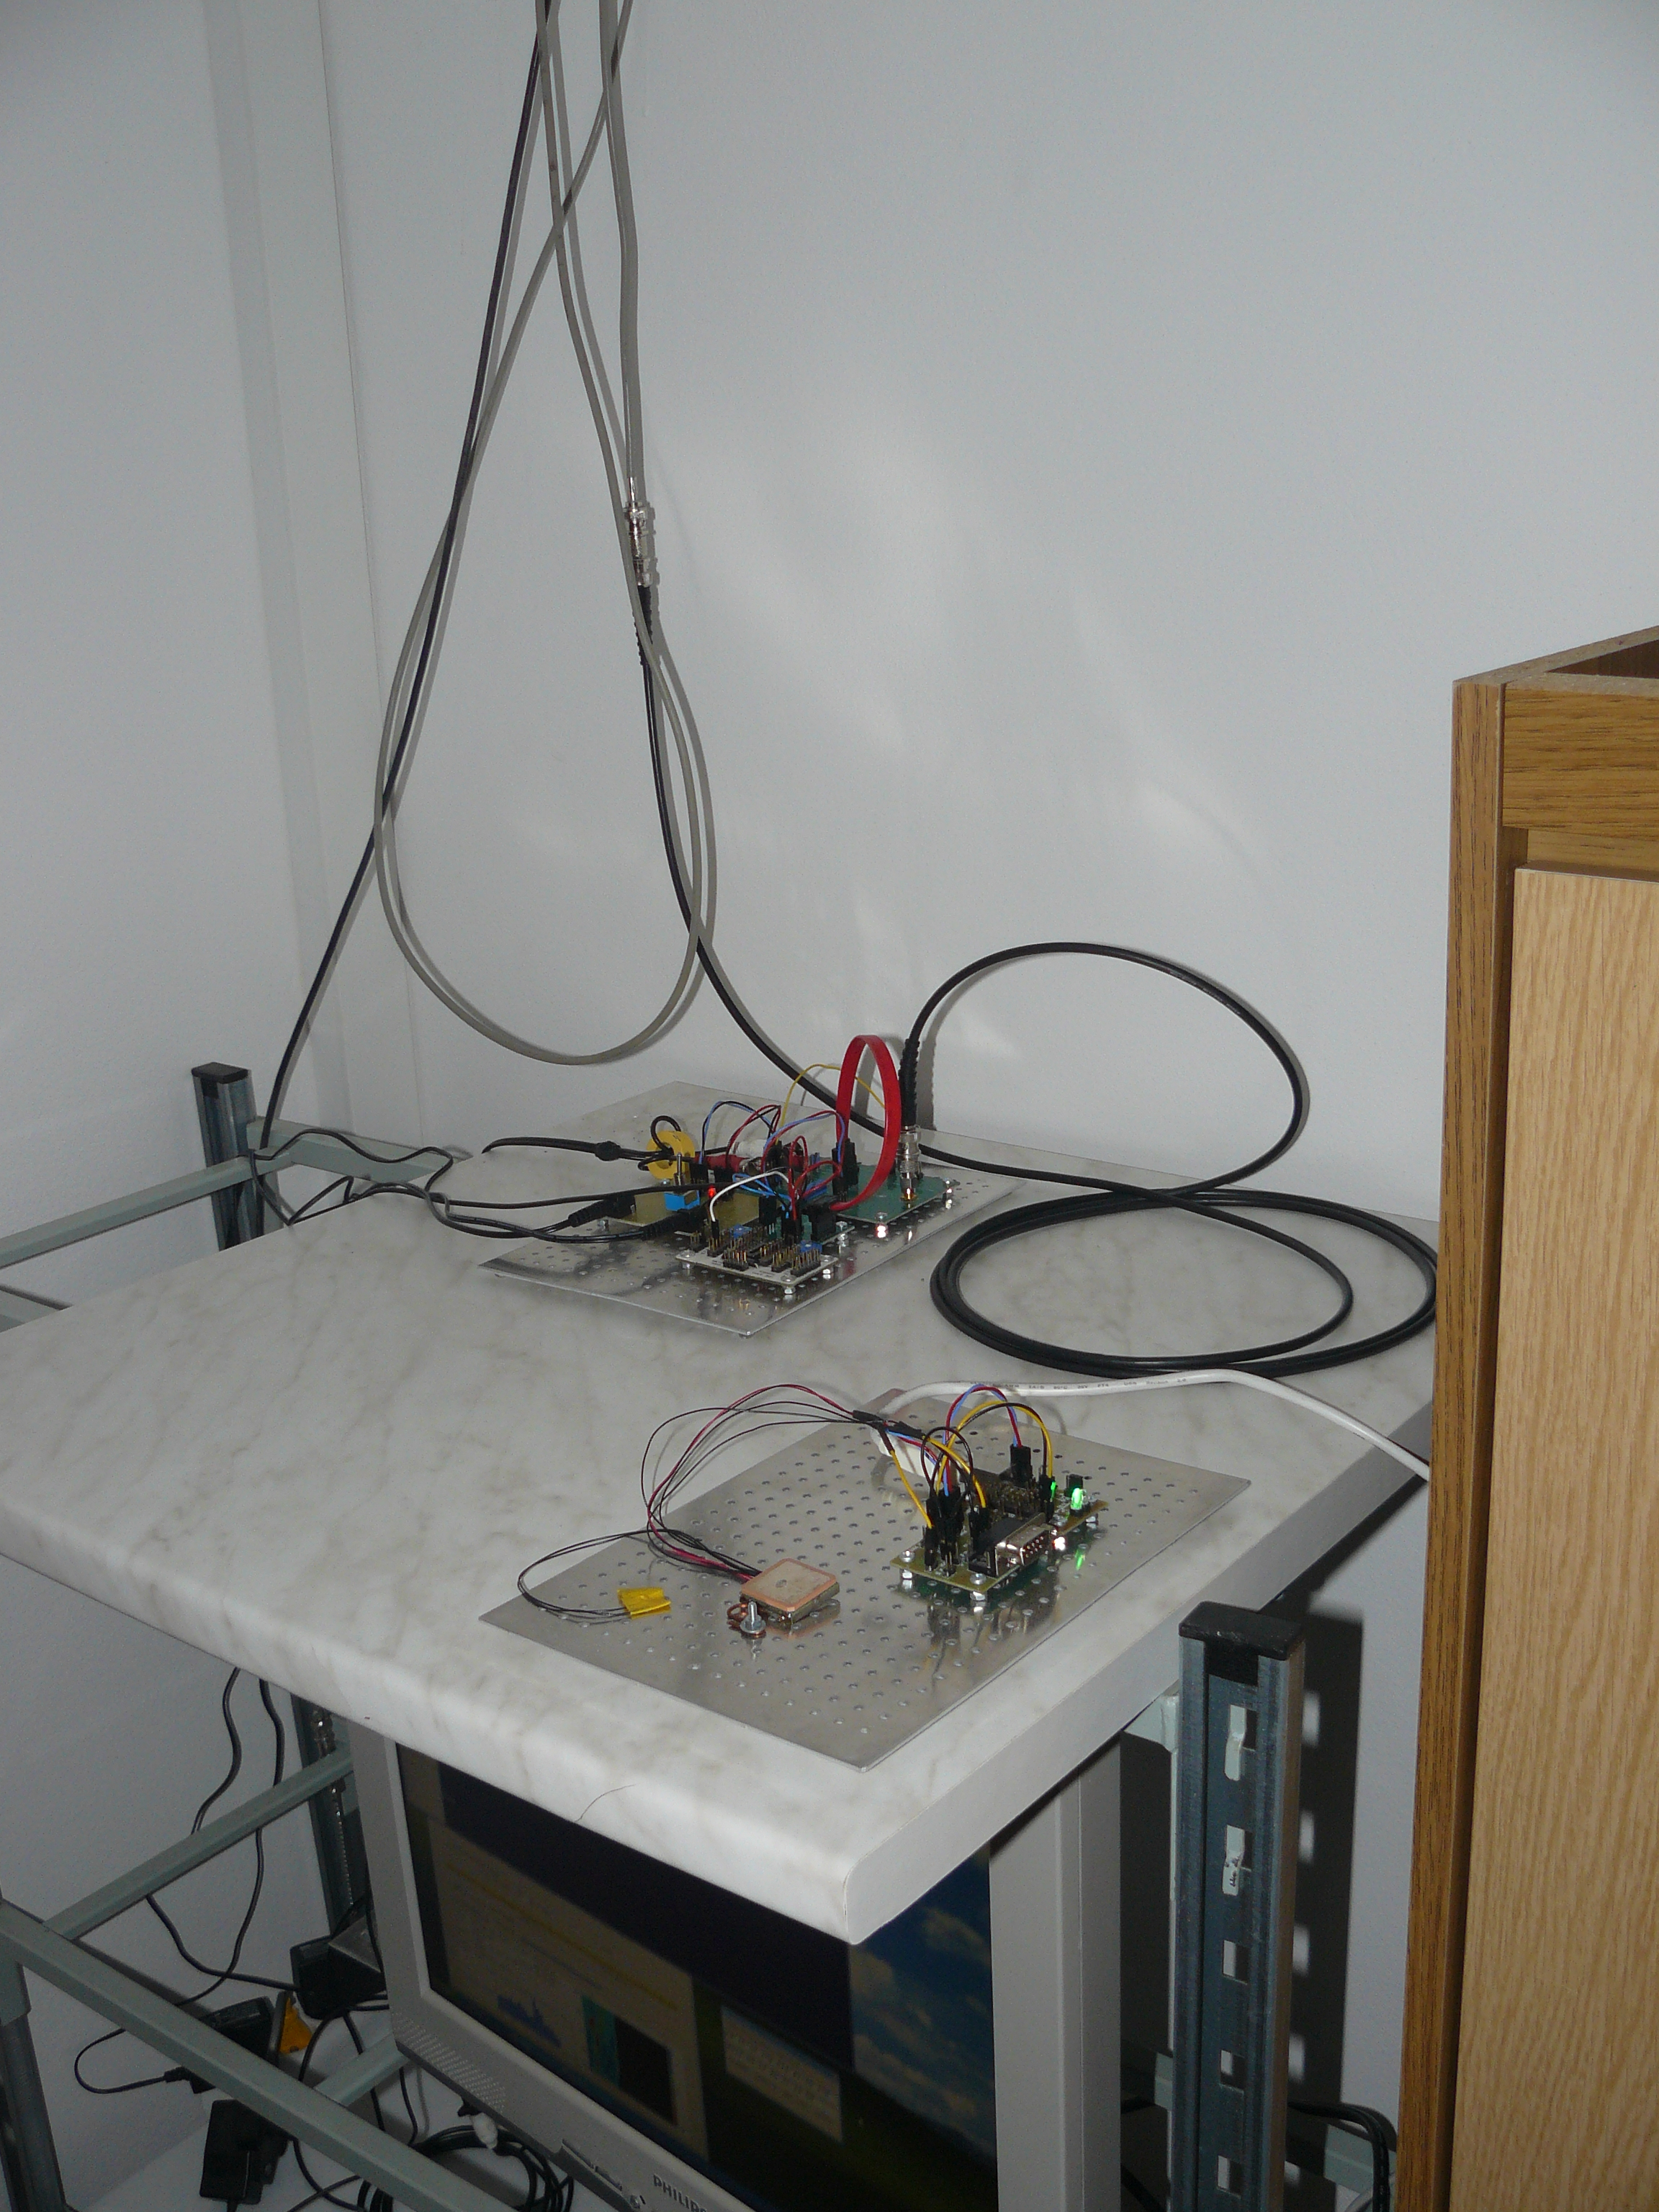
\includegraphics [width=80mm] {./img/meteor-detector_receiver.JPG} 
\end{center}
\caption{Example of meteor detector receiver setup}
\end{figure}


\begin{figure} [htbp]
\begin{center}
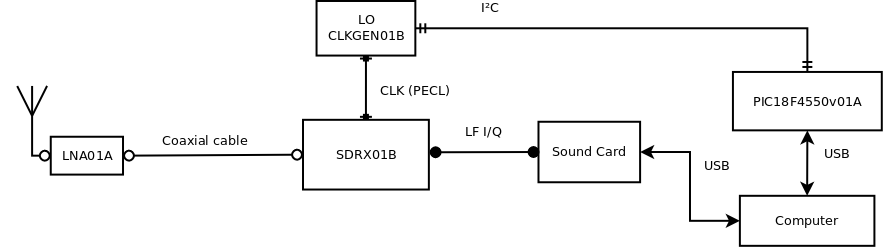
\includegraphics [width=150mm] {./img/RMDS01A_system.png} 
\end{center}
\caption{Schematic drawing of complete meteor detector}
\end{figure}


\subsection{Time synchronisation}

Time synchronisation has crucial importance in any modern science measurement. There is possibility of using many synchronisation techniques. Such as NTP or GPS (see for our article at  for our experiences)

Suggested method for time synchronisation of a measuring station depends on level of desired information which would be obtained from meteor reflection event.    

For example: If we need hour count data only. We can use PC system time without any synchronisation. But if we have one more station and we would like to compare data with another stations then NTP syncing would be good choice.  Highest level is trail parameters determination which need true radar signal processing  and most precise time synchronisation which could be achieved by GPS receiver.

\begin{figure}[htbp]
\begin{center}
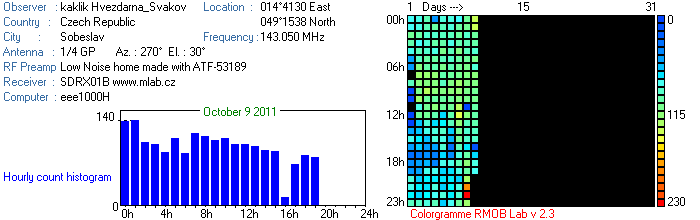
\includegraphics [width=150mm] {./img/colorgram.png} 
\end{center}
\caption{Example of measured hourly count of meteor showers}   
\end{figure}

\section{Software setup}

For simple PC based monitor station we are using SpectrumLab software with   our configuration and detection script. 

Local oscillator of SDRX01B is a CLKGEN01B module with frequency tuning controller  PIC18F4550v01A can be set up from PC or can be programmed for fixed start up frequency. If fixed start up frequency is correctly saved the only step for tuning the LO is provide power trough USB cable from PC and then press the RESET button of tuning microcomputer module. After that the LO shout be tuned on saved start up frequency. This frequency can be changed by   

\begin{thebibliography}{99}
\bibitem{Spectrum_lab}{Spectrum Lab} 
\href{http://www.qsl.net/dl4yhf/spectra1.html}{http://www.qsl.net/dl4yhf/spectra1.html}

\bibitem{Radio_meteor_detection}{Radio Meteor Detection} 
\href{http://www.gb2nlo.org/index.php/articles/meteordet}{http://www.gb2nlo.org/index.php/articles/meteordet}

\bibitem{meteor_distance}{Meteor distance parameters} 
\href{http://www.amsmeteors.org/richardson/distance.html}{http://www.amsmeteors.org/richardson/distance.html}




\end{thebibliography}
\end{document}